\chapter{COMPOSIÇÃO DA OBRA}

Devido a alta precisão para captar objetos e movimentos optou-se pelo uso do sensor Microsoft Kinect que, conectado a um computador, é responsável por captar a área onde os espectadores se encontram. Integrando-o a uma placa Arduino é possível controlar uma série de LEDs, dispostos em uma grade pendente ao teto. Cada LED possui cabos de fibra ótica side light (com emissão de luz lateral) conectados à ele que se iluminam conforme os espectadores caminham sob a grade. Na figura \ref{fig:esquema} podemos ver um esquema de montagem da obra, sendo que, o sensor Kinect fica preso junto ao teto, a grade com os LEDs se encontra abaixo, a pouco mais de 1 metro de distância, deixando espaço suficiente para os transeuntes.

\begin{figure}[H]
    \centering
    \caption{Esquema de montagem da obra. (falta computador e arduino)}
	\vspace*{0,2cm}
    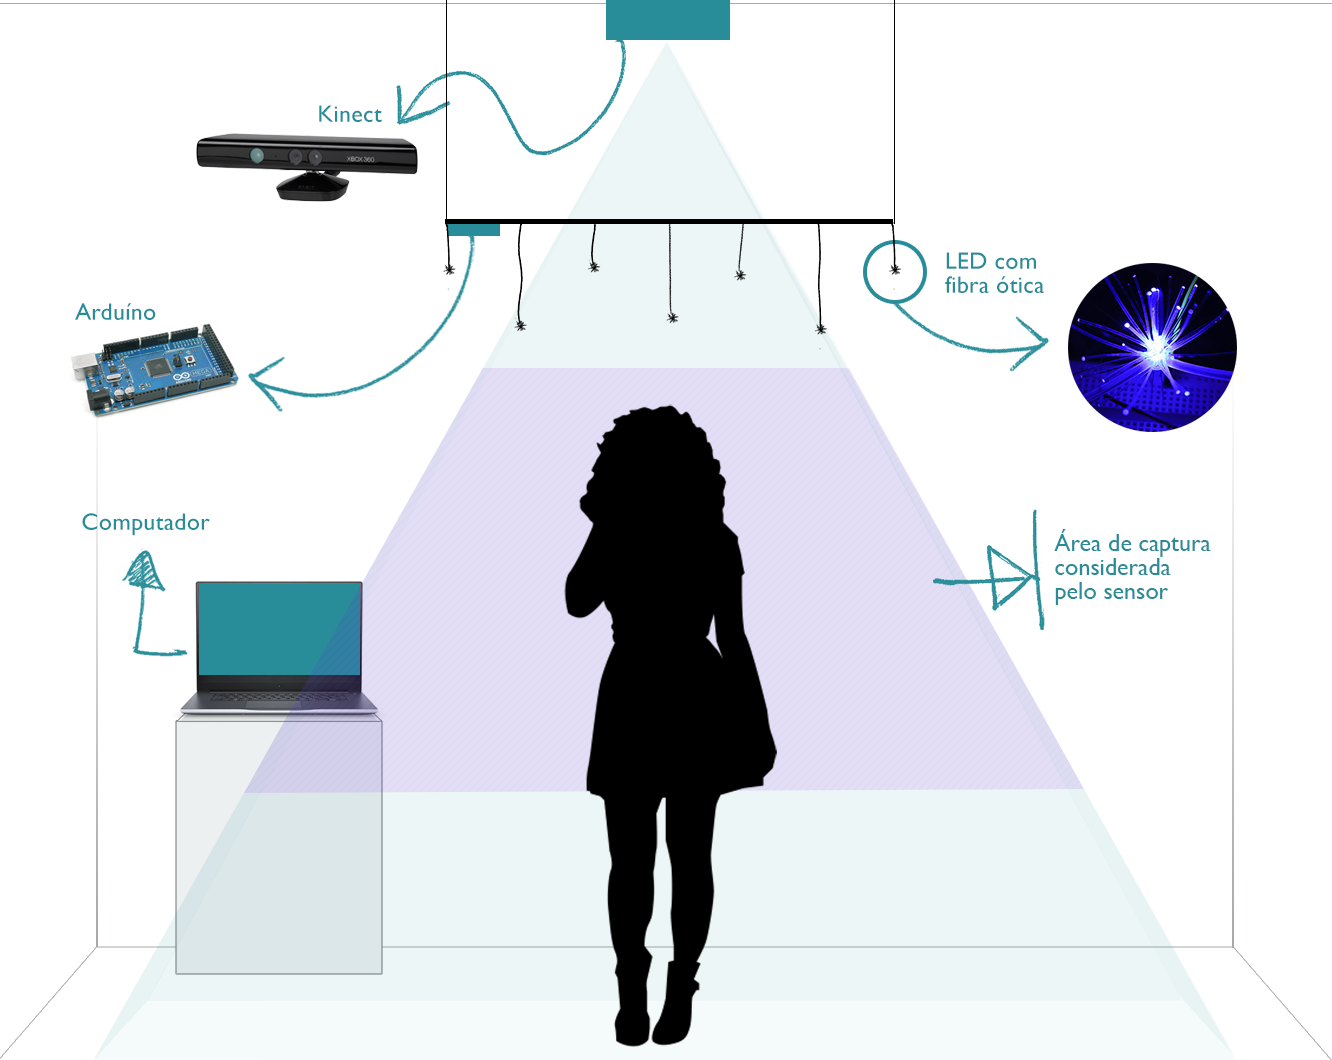
\includegraphics[width=0.8\textwidth]{./04-figuras/esquema}
    \label{fig:esquema}
\end{figure}
\vspace*{-0,9cm}
{\raggedright \fonte{Elaborada pelo autor}}\\

A seguir veremos um detalhamento de cada componente para a composição da obra, bem como aprofundaremos sobre o papel de cada um neste trabalho. 

\section{MICROSOFT KINECT}

O sensor Kinect é um dispositivo lançado em 4 de Novembro de 2010 como um acessório do console Xbox 360 da Microsoft. Orientado, principalmente, a indústria de jogos, foi criado para servir como uma forma de interação entre o utilizador e o console Xbox 360 através de gestos e comandos de voz. De acordo com a Microsoft (2018), em sua primeira versão, é capaz de capturar imagens com 640x480 pixels a 30 fps. O aparelho é formado por um sensor de profundidade, uma câmera RGB, um acelerómetro, um motor e uma série de 4 microfones. Na figura \ref{fig:kinect_componentes} podemos ver a posição de cada um destes componentes no dispositivo.

\begin{figure}[H]
    \centering
    \caption{Componentes do sensor Kinect}
	\vspace*{0,2cm}
    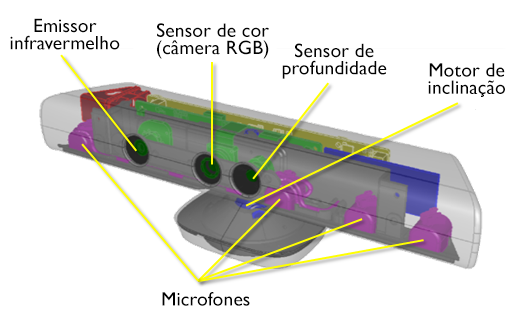
\includegraphics[width=0.8\textwidth]{./04-figuras/kinect_componentes}
    \label{fig:kinect_componentes}
\end{figure}
\vspace*{-0,9cm}
{\raggedright \fonte{Microsoft (2008)}}\\

Dentre seus componentes, o que mais nos interessa no contexto deste trabalho, é o sensor de profundidade. Ashley e Webb \cite{ashley} afirmam que a produção de dados tridimensionais é a principal função do Kinect. Ele difere de qualquer outro dispositivo de entrada justamente porque provê uma terceira dimensão e, para tanto, se utiliza de um emissor e uma câmera de infravermelho. Segundo Lucero (2012) o emissor de infravermelhos projeta um padrão estruturado de luz infravermelha, enquanto a câmera lê esses raios e interpreta a deformação da projeção, convertendo essa informação em valores de profundidade e, consequentemente, medindo a distância entre o objeto e o sensor. De acordo com Correia (2013) estas medidas baseiam-se em triangulação tendo em conta o emissor, a câmera e as posições dos pixels no cenário. A profundidade é codificada numa escala de cinzas. Quanto mais escuro o pixel, mais próximo do sensor está esse ponto no espaço. Sendo que, pixels pretos indicam que não existe informação de profundidade. Isto ocorre no caso dos pontos estarem muito longe, impossibilitando a sua captura, no caso de estarem numa área onde não haja pontos do emissor de infravermelhos, no caso de o objeto refletir mal a luz infravermelha ou, finalmente, no caso de os pontos estarem muito próximos do sensor, uma vez que o campo de visão do Kinect é limitado em cerca de 80 centímetros a 4 metros.

Considerando as limitações do sensor Kinect, a que mais impactou este projeto, é causada pela própria natureza da luz projetada pelo sensor. A luz emitida pelo projetor de infravermelho, ao se deparar com um objeto, gera uma sombra em outro que esteja numa distância maior. Segundo Lucero (2013) o resultado é que não se pode determinar a profundidade em zonas afetadas por estas sombras, como pode ser visto na figura \ref{fig:kinect_sombras}. Dessa forma, estas sombras criam zonas negras na imagem de profundidade, ou seja, pixels com valor zero. O impacto gerado aqui é devido à malha de LEDs se encontrar entre o sensor Kinect e o espectador. A malha projeta uma sombra, criando pontos onde o espectador pode não ser percebido.  Mais detalhes sobre essa questão serão vistos na seção 5.3 Malha de LEDs e fibra ótica.

\begin{figure}[H]
    \centering
    \caption{Efeito das sombras no sensor Kinect}
	\vspace*{0,2cm}
    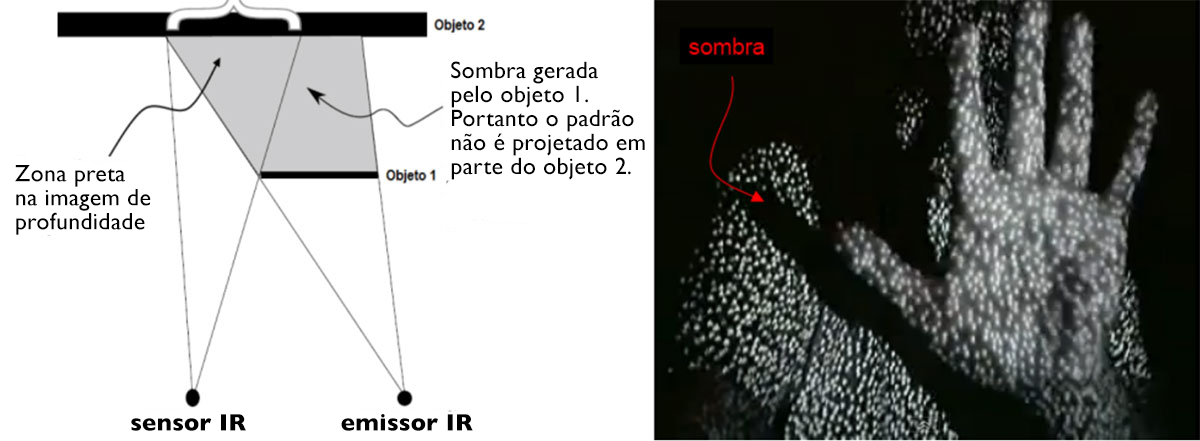
\includegraphics[width=0.8\textwidth]{./04-figuras/kinect_sombras}
    \label{fig:kinect_sombras}
\end{figure}
\vspace*{-0,9cm}
{\raggedright \fonte{Lucero (2013)}}\\


O Microsoft Kinect foi utilizado como fonte de entrada de dados para mapear o ambiente tridimensional e com ajuda da Processing\footnote{Processing é uma plataforma e uma linguagem de programação para prototipação de software dentro do contexto das artes visuais. Desde 2001, a Processing promoveu a alfabetização em software dentro das artes visuais e a alfabetização visual dentro da tecnologia. Há dezenas de milhares de estudantes, artistas, designers, pesquisadores e amadores que usam Processing para aprender e criar protótipos (PROCESSING, 2018).} criar uma malha bidimensional que, mais tarde, é transferida para a estrutura de LEDs. A figura \ref{fig:kinect_exemplo} mostra um exemplo de imagem gerada a partir dos dados capturados pelo sensor. Cada ponto branco apresentado na figura representa um LED aceso na estrutura física, enquanto a área em preto demarca os intervalos entre os mesmos. Não há distinção, na imagem, entre os intervalos e os LEDs apagados. 

\begin{figure}[H]
    \centering
    \caption{Exemplo de imagem gerada a partir  das informações capturadas  pelo sensor Kinect.}
	\vspace*{0,2cm}
    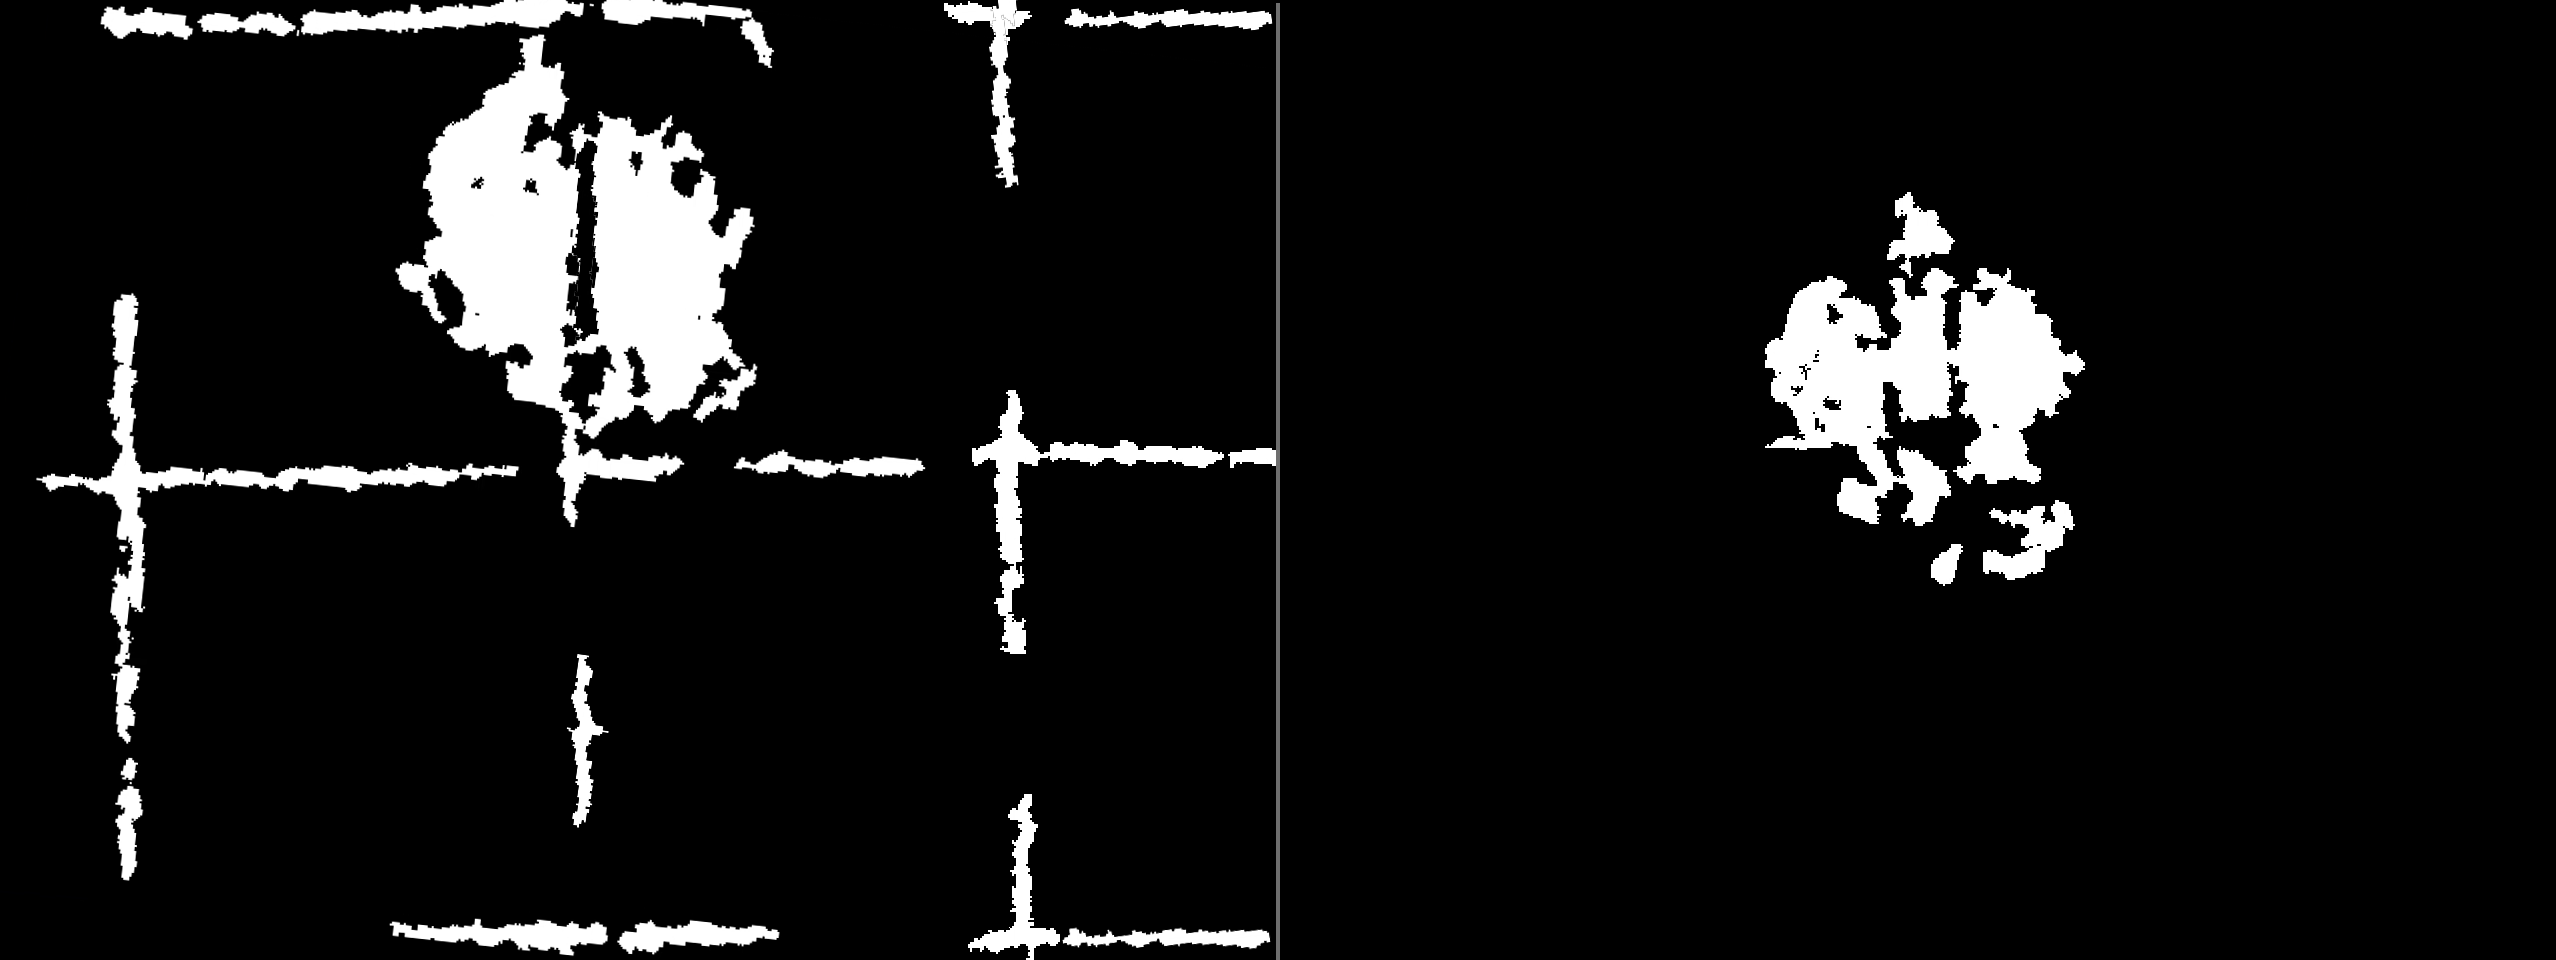
\includegraphics[width=0.8\textwidth]{./04-figuras/kinect_exemplo}
    \label{fig:kinect_exemplo}
\end{figure}
\vspace*{-0,9cm}
{\raggedright \fonte{Captura de tela de imagem gerada pelo sensor Kinect}}\\


\section{ARDUINO}

Antes de detalhar o papel do Arduino na obra, propõe-se o entendimento do que é e para que serve, para tanto podemos analisar a descrição presente no site oficial do projeto:

\begin{citacao}
Arduino é uma plataforma de prototipagem eletrônica de hardware livre e de placa única. O objetivo do projeto é criar ferramentas que são acessíveis, com baixo custo, flexíveis e fáceis de usar. Placas arduíno são capazes de ler uma entrada como a luz em um sensor, um dedo pressionando um botão ou uma mensagem do Twitter e transformá-la em uma saída como ativar um motor, ligar um LED ou publicar alguma coisa na internet, por exemplo. É possível dizer à placa o que fazer enviando uma série de instruções ao microcontrolador. Para isso é necessário utilizar a linguagem de programação do Arduino (baseada em Wiring) e o seu software (IDE), baseada em Processing \cite{arduino}. 
\end{citacao}

Neste trabalho o Arduino foi utilizado para controlar os circuitos da malha de LEDs (saída) recebendo as informações mapeadas pelo sensor Kinect (entrada). Cada LED precisa ser controlado individualmente, por isso optou-se pela utilização do Arduino Mega que possui 54 entradas/saídas digitais, sendo a placa disponível com o maior número de entradas/saídas.


\section{MALHA DE LEDS E FIBRA ÓTICA}

Uma malha de LEDs será construída equivalente a área de captura do Kinect a uma distância de pouco mais de 1 metro do teto.
